\documentclass[11pt,letterpaper]{report}

\usepackage[utf8]{inputenc}
\usepackage[T1]{fontenc}
\usepackage[spanish,provide=*]{babel}
\usepackage{amsmath,amssymb}
\usepackage{booktabs}
\usepackage{array}
\usepackage{graphicx}
\usepackage{float}
\usepackage{caption}
\usepackage{tikz}
\usetikzlibrary{arrows.meta}
\usepackage[margin=2.5cm]{geometry}
\usepackage{enumitem}
\usepackage{siunitx}

\renewcommand{\arraystretch}{1.15}

\begin{document}

\begin{center}
{\LARGE\bfseries\linespread{1.3}\selectfont 3. PRUEBAS ESTADÍSTICAS PARA LOS NÚMEROS PSEUDOALEATORIOS\par}
\end{center}
\vspace{0.5cm}

\setcounter{chapter}{3}
\setcounter{page}{31}

%==========================================================
Puesto que cualquier variable aleatoria no-uniforme (normal, exponencial,
poisson, etc.), es obtenida a partir de números uniformes $(0;1)$, el
principal énfasis en pruebas estadísticas deberá ser con respecto al
generador de números pseudoaleatorios, ya que cualquier deficiencia
estadística en la distribución de la variable aleatoria no-uniforme, se
deberá exclusivamente a la utilización de un deficiente generador de
números pseudoaleatorios. Por consiguiente, en el presente capítulo se
explican algunas de las muchas pruebas estadísticas que han sido
desarrolladas para probar la aleatoriedad de los números pseudoaleatorios.

%==========================================================
\section*{3.1. Prueba de los promedios}

Quizá la función de densidad de probabilidad más simple es aquella que
se caracteriza por ser constante en el intervalo $(0;1)$ y cero fuera de
él (ver figura 3.1). Esta función de densidad define la distribución
conocida como uniforme o rectangular. Matemáticamente, la función de
densidad uniforme se define como:

\[
f(x) = \begin{cases} 1 & \text{si } 0 \le x \le 1 \\ 0 & \text{si } 0 > x > 1 \end{cases}
\]

En esta expresión, $x$ es una variable aleatoria definida en el
intervalo $(0;1)$. Por otra parte, la distribución acumulada $F(x)$, de
una variable aleatoria $x$ uniformemente distribuida, se puede obtener
como:

\begin{equation}
F(x) = \int_0^x 1\,dt = x
\end{equation}

El valor esperado y la varianza de una variable aleatoria uniformemente
distribuida están dadas por las siguientes expresiones:

\begin{equation}
E(x) = \int_0^1 x(1)\,dx = \frac{1}{2}
\end{equation}

\begin{equation}
\text{var}(x) = \int_0^1 (x-1/2)^2 (1)\,dx = 1/12
\end{equation}

\begin{figure}[H]
\centering
\begin{tikzpicture}[scale=2]
  \draw[-{Latex}] (-0.3,0) -- (1.6,0) node[right]{$x$};
  \draw[-{Latex}] (0,-0.2) -- (0,1.4) node[above]{$f(x)$};
  \draw[thick] (0,1) -- (1,1);
  \draw[dashed] (0,1) -- (0,0);
  \draw[dashed] (1,1) -- (1,0);
  \node[left] at (0,1) {1};
  \node[below] at (1,0) {1};
\end{tikzpicture}
\hspace{1.5cm}
\begin{tikzpicture}[scale=2]
  \draw[-{Latex}] (-0.3,0) -- (1.6,0) node[right]{$x$};
  \draw[-{Latex}] (0,-0.2) -- (0,1.4) node[above]{$F(x)$};
  \draw[thick] (0,0) -- (1,1);
  \draw[dashed] (0,1) -- (1,1);
  \draw[dashed] (1,1) -- (1,0);
  \node[left] at (0,1) {1};
  \node[below] at (1,0) {1};
\end{tikzpicture}
\caption*{\textbf{Figura 3.1} Distribución de probabilidad y distribución acumulada de los números uniformes $(0;1)$}
\end{figure}

Conociendo los parámetros de la distribución uniforme, es posible
plantear una prueba de hipótesis de promedios, con la cual se trata de
probar que los números pseudoaleatorios generados provienen de un
universo uniforme con media de 0.5. Más específicamente, una prueba de
hipótesis de promedios puede ser planteada de la siguiente forma:

\begin{align*}
\text{Hipótesis nula } H_0&: u = 1/2 \\
\text{Hipótesis alternativa } H_1&: u \ne 1/2
\end{align*}

La realización de esta prueba requiere obtener una muestra de tamaño
$N$, es decir, es necesario generar $N$ números pseudoaleatorios. En
seguida, su promedio aritmético es evaluado de acuerdo a la siguiente
expresión:

\begin{equation}
\bar{x} = \frac{U_1 + U_2 + \ldots + U_N}{N}
\end{equation}

En seguida se determina el valor del estadístico $Z_0$, utilizando la
siguiente expresión:

\begin{equation}
Z_0 = \frac{(\bar{x} - 1/2)\sqrt{N}}{\sqrt{1/12}}
\end{equation}

Si $|Z_0| < Z_{\alpha/2}$, entonces no se puede rechazar la hipótesis de
que los números pseudoaleatorios generados provienen de un universo
uniforme con media de 0.5.

Para ilustrar la aplicación de esta prueba de hipótesis, considere los
números pseudoaleatorios presentados en la tabla 3.1. Para estos
números, la media aritmética resulta ser de 0.48234, y el estadístico
$Z_0$ resulta ser de:

\begin{equation}
Z_0 = \frac{(0.48234 - 0.5)\sqrt{100}}{\sqrt{1/12}} = -0.61
\end{equation}

Si se supone un nivel de significado ($\alpha$) de 5\%, entonces
$Z_{\alpha/2}$ tiene un valor de 1.96 y puesto que $|Z_0| < 1.96$,
entonces no se puede rechazar la hipótesis de que estos números
pseudoaleatorios tienen una media de 0.5.

\begin{table}[H]
\centering
\caption*{\textbf{Tabla 3.1} Tabla de números pseudoaleatorios}
\begin{tabular}{*{5}{S[table-format=1.5]}}
\toprule
0.78961 & 0.05230 & 0.10699 & 0.55877 & 0.14151 \\
0.76086 & 0.12079 & 0.27738 & 0.65726 & 0.79269 \\
0.80548 & 0.82654 & 0.29453 & 0.20852 & 0.42989 \\
0.58518 & 0.98611 & 0.34488 & 0.34358 & 0.11537 \\
0.89898 & 0.57880 & 0.67621 & 0.05010 & 0.00121 \\
0.28269 & 0.73059 & 0.70119 & 0.18284 & 0.49962 \\
0.38618 & 0.76910 & 0.68334 & 0.55170 & 0.10850 \\
0.79982 & 0.45679 & 0.21631 & 0.87616 & 0.55743 \\
0.58962 & 0.33216 & 0.03185 & 0.61168 & 0.09264 \\
0.69623 & 0.17028 & 0.05475 & 0.91512 & 0.76262 \\
0.29931 & 0.30861 & 0.83358 & 0.51781 & 0.03272 \\
0.57410 & 0.26593 & 0.85903 & 0.43308 & 0.35286 \\
0.24000 & 0.65559 & 0.38507 & 0.90829 & 0.94187 \\
0.93655 & 0.88809 & 0.81772 & 0.36982 & 0.19904 \\
0.54325 & 0.62400 & 0.09133 & 0.41678 & 0.33954 \\
0.58244 & 0.85853 & 0.88752 & 0.33729 & 0.15506 \\
0.23949 & 0.53559 & 0.33381 & 0.49383 & 0.75103 \\
0.19962 & 0.65002 & 0.74579 & 0.79113 & 0.63453 \\
0.19147 & 0.40644 & 0.08128 & 0.73435 & 0.22724 \\
0.22287 & 0.07281 & 0.64183 & 0.44267 & 0.72102 \\
\bottomrule
\end{tabular}
\end{table}

%==========================================================
\section*{3.2. Prueba de frecuencias}

Probablemente una de las más importantes pruebas sobre aleatoriedad de
los números pseudoaleatorios es la prueba de las frecuencias. Esta
prueba consiste en dividir el intervalo $(0;1)$ en $n$ subintervalos
(ver figura 3.2) para luego comparar para cada subintervalo la
frecuencia esperada con la frecuencia observada. Si estas frecuencias
son bastante parecidas, entonces la muestra proviene de una distribución
uniforme. El estadístico que se usa en esta prueba es $X_0^2$ el cual se
obtiene de acuerdo a la siguiente expresión:

\begin{equation}
X_0^2 = \sum_{i=1}^{n} \frac{(FO_i - FE_i)^2}{FE_i}
\end{equation}

donde:
\begin{align*}
FO_i &= \text{Frecuencia observada del } i\text{-ésimo subintervalo.} \\
FE_i &= \text{Frecuencia esperada del } i\text{-ésimo subintervalo } (N/n). \\
N &= \text{Tamaño de la muestra.} \\
n &= \text{Número de subintervalos.}
\end{align*}

\begin{figure}[H]
\centering
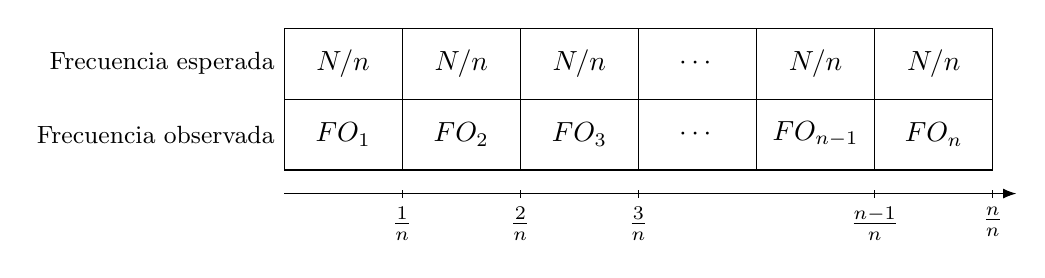
\begin{tikzpicture}[scale=1]
  \def\w{1.5}
  \def\h{0.9}
  \foreach \i in {0,...,6} {
    \draw (\i*\w,0) -- (\i*\w,2*\h);
  }
  \draw (0,0) -- (6*\w,0);
  \draw (0,\h) -- (6*\w,\h);
  \draw (0,2*\h) -- (6*\w,2*\h);
  \node[left] at (0,1.5*\h) {\small Frecuencia esperada};
  \node[left] at (0,0.5*\h) {\small Frecuencia observada};
  \node at (0.5*\w,1.5*\h) {$N/n$};
  \node at (1.5*\w,1.5*\h) {$N/n$};
  \node at (2.5*\w,1.5*\h) {$N/n$};
  \node at (3.5*\w,1.5*\h) {$\cdots$};
  \node at (4.5*\w,1.5*\h) {$N/n$};
  \node at (5.5*\w,1.5*\h) {$N/n$};
  \node at (0.5*\w,0.5*\h) {$FO_1$};
  \node at (1.5*\w,0.5*\h) {$FO_2$};
  \node at (2.5*\w,0.5*\h) {$FO_3$};
  \node at (3.5*\w,0.5*\h) {$\cdots$};
  \node at (4.5*\w,0.5*\h) {$FO_{n-1}$};
  \node at (5.5*\w,0.5*\h) {$FO_n$};
  \draw[-{Latex}] (0,-0.3) -- (6*\w+0.3,-0.3);
  \draw (1*\w,-0.35) -- (1*\w,-0.25);
  \draw (2*\w,-0.35) -- (2*\w,-0.25);
  \draw (3*\w,-0.35) -- (3*\w,-0.25);
  \draw (5*\w,-0.35) -- (5*\w,-0.25);
  \draw (6*\w,-0.35) -- (6*\w,-0.25);
  \node[below] at (1*\w,-0.35) {$\frac{1}{n}$};
  \node[below] at (2*\w,-0.35) {$\frac{2}{n}$};
  \node[below] at (3*\w,-0.35) {$\frac{3}{n}$};
  \node[below] at (5*\w,-0.35) {$\frac{n-1}{n}$};
  \node[below] at (6*\w,-0.35) {$\frac{n}{n}$};
\end{tikzpicture}
\caption*{\textbf{Figura 3.2} Frecuencia esperada y observada de cada subintervalo}
\end{figure}

Este estadístico $X_0^2$ se compara con $X^2_{\alpha,(n-1)}$, la cual
representa a una variable aleatoria chi-cuadrada con $(n-1)$ grados de
libertad y un nivel de significado $\alpha$. Si $X_0^2 <
X^2_{\alpha,(n-1)}$, entonces no se puede rechazar la hipótesis de que
la muestra proviene de una distribución uniforme.

Por ejemplo, si se aplica esta prueba a los números pseudoaleatorios
presentados en la tabla 3.1, y además considere que el número de
subintervalos es 5, es decir, $n=5$. Para este valor de $n$, la
frecuencia esperada de cada subintervalo es 20, y las frecuencias
observadas son:

\begin{table}[H]
\centering
\begin{tabular}{cccccc}
\toprule
 & \multicolumn{5}{c}{Subintervalo (.2, .4, .6, .8, 1)} \\
\midrule
Frecuencia esperada & 20 & 20 & 20 & 20 & 20 \\
Frecuencia observada & 21 & 22 & 19 & 23 & 15 \\
\bottomrule
\end{tabular}
\end{table}

Por consiguiente, aplicando la ecuación anterior se obtiene:

\begin{equation}
X_0^2 = \frac{1}{20}\left\{ (21-20)^2 + (22-20)^2 + (19-20)^2 + (23-20)^2 + (15-20)^2 \right\} = 2
\end{equation}

Si se especifica un valor arbitrario de $\alpha = 0.05$, entonces
$X^2_{0.05,4} = 9.49$. Puesto que $X_0^2 < X^2_{0.05,4}$, entonces no se
puede rechazar la hipótesis de que los números pseudoaleatorios
presentados en la tabla 3.1 provienen de una distribución uniforme.

%==========================================================
\section*{3.3. Prueba de la distancia}

Esta prueba puede ser realizada de dos maneras: considerando a los
números pseudoaleatorios generados como dígitos, o considerando como
números reales.

\subsection*{3.3.1. Números pseudoaleatorios considerados como dígitos}

Si los números pseudoaleatorios generados son considerados como
dígitos, entonces la prueba consiste en contar el número de dígitos que
aparece entre ocurrencias sucesivas de un mismo dígito. Por ejemplo,
58245 ilustra un hueco de tamaño 3 entre los dos cincos.

La probabilidad de cada uno de los tamaños de hueco ($i=0,1,2,\ldots$)
se obtiene con la siguiente expresión:

\begin{equation}
P_i = 0.1(0.9)^i \quad \text{para } i = 0, 1, 2, \ldots
\end{equation}

Sin embargo, como teóricamente el valor del tamaño del hueco puede ser
infinito, es conveniente agrupar las probabilidades para valores de $i$
mayores o iguales a un determinado valor de $n$. Tal sumatoria se
obtiene de acuerdo a la siguiente expresión:

\begin{equation}
P_{i \ge n} = \sum_{m=0}^{\infty} 0.1(0.9)^{m+n} = (0.9)^n
\end{equation}

Con las ecuaciones anteriores se obtienen las frecuencias esperadas para
cada tamaño de hueco. La obtención de tales frecuencias se ilustra en la
tabla 3.2. Si las frecuencias esperadas y observadas para cada tamaño de
hueco son bastante parecidas, entonces se puede decir que los números
pseudoaleatorios generados pasan la prueba de la distancia. El
estadístico $X_0^2$ que se usa en esta prueba se obtiene como:

\begin{equation}
X_0^2 = \sum_{i=0}^{n} \frac{(FO_i - FE_i)^2}{FE_i}
\end{equation}

el cual se compara con $X^2_{\alpha,n}$. Si $X_0^2 < X^2_{\alpha,n}$,
entonces los números pseudoaleatorios pasan la prueba de la distancia.
Es muy importante señalar que el valor seleccionado de $n$, debe ser tal
que la suma de las frecuencias esperadas de todos los tamaños de huecos
agrupados, sea mayor que 5.

\begin{table}[H]
\centering
\caption*{\textbf{Tabla 3.2} Frecuencias esperadas y observadas para los diferentes tamaños de hueco, considerando a los números pseudoaleatorios generados como dígitos}
\begin{tabular}{cccc}
\toprule
$i$ & $P_i$ & $FO_i$ & $FE_i$ \\
\midrule
0 & 0.1 & $FO_0$ & $\Sigma FO_i (0.1)$ \\
1 & $0.1(0.9)$ & $FO_1$ & $\Sigma FO_i (0.1)(0.9)$ \\
2 & $0.1(0.9)^2$ & $FO_2$ & $\Sigma FO_i (0.1)(0.9)^2$ \\
$\vdots$ & $\vdots$ & $\vdots$ & $\vdots$ \\
$i$ & $0.1(0.9)^i$ & $FO_i$ & $\Sigma FO_i (0.1)(0.9)^i$ \\
$\vdots$ & $\vdots$ & $\vdots$ & $\vdots$ \\
$\ge n$ & $(0.9)^n$ & $FO_n$ & $\Sigma FO_i (0.9)^n$ \\
\midrule
Total & 1.0 & $\Sigma FO_i$ & $\Sigma FO_i$ \\
\bottomrule
\end{tabular}
\end{table}

\subsection*{3.3.2. Números pseudoaleatorios considerados como números reales}

Si los números pseudoaleatorios generados son considerados como números
reales, entonces, para realizar esta prueba es necesario seleccionar un
intervalo $(\alpha;\beta)$, el cual debe de estar contenido en el
intervalo $(0;1)$, es decir, $0 \le \alpha \le \beta \le 1$. En seguida,
para cada número pseudoaleatorio generado se pregunta si es o no
elemento del intervalo $(\alpha;\beta)$. Si $U_j$ (número uniforme
generado) es elemento de $(\alpha;\beta)$, $U_{j+1}$ hasta $U_{j+i}$ no
son elementos de dicho intervalo y $U_{j+i+1}$ vuelve a ser elemento del
intervalo $(\alpha;\beta)$, entonces se tiene un hueco de tamaño $i$.
Por ejemplo, si $\alpha = .3$ y $\beta = .5$ y los números
pseudoaleatorios generados son como sigue: 0.32415, 0.22257, 0.19147,
0.75103, 0.49383, entonces el hueco es de tamaño 3.

Para el caso de considerar los números pseudoaleatorios generados como
números reales, la distribución de probabilidad del tamaño del hueco es
como sigue:

\begin{equation}
P_i = \theta(1-\theta)^i \quad \text{para } i = 0, 1, 2, \ldots
\end{equation}

donde $\theta = \beta - \alpha$ representa la probabilidad de caer en el
intervalo $(\alpha;\beta)$.

Al igual que en el inciso anterior, es conveniente agrupar las
probabilidades para valores de $i \ge n$. Tal agrupación se obtiene con
la siguiente expresión:

\begin{equation}
P_{i \ge n} = \sum_{m=0}^{\infty} \theta(1-\theta)^{m+n} = (1-\theta)^n
\end{equation}

Con las ecuaciones anteriores se obtienen las frecuencias esperadas, las
cuales aparecen en la tabla 3.3. Utilizando el estadístico $X_0^2$ y
comparando el resultado obtenido con $X^2_{\alpha,n}$, se toma la
decisión de aceptar o rechazar la prueba de la distancia. Es muy
importante señalar que el valor de $\alpha$ y $\beta$ no tienen ninguna
influencia en la bondad de la prueba, y también es necesario señalar que
el valor de $n$ debe ser seleccionado de acuerdo al criterio mencionado
en el inciso anterior.

\begin{table}[H]
\centering
\caption*{\textbf{Tabla 3.3} Frecuencias esperadas y observadas para los diferentes tamaños de hueco, considerando a los números pseudoaleatorios generados como números reales}
\begin{tabular}{cccc}
\toprule
$i$ & $P_i$ & $FO_i$ & $FE_i$ \\
\midrule
0 & $\theta$ & $FO_0$ & $\Sigma FO_i (\theta)$ \\
1 & $\theta(1-\theta)$ & $FO_1$ & $\Sigma FO_i (\theta)(1-\theta)$ \\
2 & $\theta(1-\theta)^2$ & $FO_2$ & $\Sigma FO_i (\theta)(1-\theta)^2$ \\
$\vdots$ & $\vdots$ & $\vdots$ & $\vdots$ \\
$i$ & $\theta(1-\theta)^i$ & $FO_i$ & $\Sigma FO_i (\theta)(1-\theta)^i$ \\
$\vdots$ & $\vdots$ & $\vdots$ & $\vdots$ \\
$\ge n$ & $(1-\theta)^n$ & $FO_n$ & $\Sigma FO_i (1-\theta)^n$ \\
\midrule
Total & 1.0 & $\Sigma FO_i$ & $\Sigma FO_i$ \\
\bottomrule
\end{tabular}
\end{table}

Por ejemplo, si se consideran los números pseudoaleatorios presentados
en la tabla 3.1, un valor de $n=3$ y valores de $\alpha=.3$ y
$\beta=.7$, entonces las frecuencias observadas y esperadas para los
diferentes tamaños de hueco serían como aparecen en la tabla 3.4. Para
estas frecuencias el valor del estadístico $X_0^2$ sería:

\begin{equation}
X_0^2 = \frac{(11-16)^2}{16} + \frac{(12-9.6)^2}{9.6} + \frac{(11-5.76)^2}{5.76} + \frac{(6-8.64)^2}{8.64} = 7.74
\end{equation}

Si se especifica un valor arbitrario de $\alpha = 0.05$, entonces
$X^2_{0.05,3} = 7.81$. Puesto que $X_0^2 < X^2_{0.05,3}$, entonces los
números pseudoaleatorios presentados en la tabla 3.1 pasan la prueba de
la distancia.

\begin{table}[H]
\centering
\caption*{\textbf{Tabla 3.4} Frecuencias esperadas y observadas para los diferentes tamaños de hueco que originan los números pseudoaleatorios presentados en la tabla 3.1}
\begin{tabular}{cccc}
\toprule
$i$ & $P_i$ & $FO_i$ & $FE_i$ \\
\midrule
0 & 0.400 & 11 & 16.00 \\
1 & 0.240 & 12 & 9.60 \\
2 & 0.144 & 11 & 5.76 \\
$\ge 3$ & 0.216 & 6 & 8.64 \\
\midrule
Total & 1.000 & 40 & 40.00 \\
\bottomrule
\end{tabular}
\end{table}

%==========================================================
\section*{3.4. Prueba de series}

La prueba de series se utiliza para comprobar el grado de aleatoriedad
entre números sucesivos. Usualmente esta prueba consiste en formar
parejas de números, las cuales son consideradas como coordenadas en un
cuadrado unitario dividido en $n^2$ celdas. Esta idea se puede extender
a las ternas de números pseudoaleatorios que representan puntos en un
cubo unitario. Sin embargo, en esta sección se analiza sólo el caso de
dos dimensiones.

La prueba de series consiste en generar $N$ números pseudoaleatorios de
los cuales se forman parejas aleatorias entre $U_i$ y $U_{i+1}$, es
decir, si se generan 10 números, entonces las parejas aleatorias que se
pueden formar serían:

\[
(U_1,U_2),\ (U_2,U_3),\ (U_3,U_4),\ (U_4,U_5),\ (U_5,U_6),\
(U_6,U_7),\ (U_7,U_8),\ (U_8,U_9),\ (U_9,U_{10})
\]

En seguida, se determina la celda a que pertenece cada pareja ordenada
(ver figura 3.3), con lo cual se determina la frecuencia observada de
cada celda. La frecuencia esperada de cada celda se obtiene al dividir
el total de parejas coordenadas $(N-1)$ por el total de celdas $(n^2)$.
Finalmente, conocida la frecuencia observada y esperada de cada celda,
se obtiene el estadístico $X_0^2$ como sigue:

\begin{equation}
X_0^2 = \frac{n^2}{N-1} \sum_{i=1}^{n} \sum_{j=1}^{n} \left( FO_{ij} - \frac{N-1}{n^2} \right)^2
\end{equation}

donde $FO_{ij}$ es la frecuencia observada de la celda $ij$. Si $X_0^2 <
X^2_{\alpha,n^2-1}$ entonces no se puede rechazar la hipótesis de que
los números provienen de una distribución uniforme.

\begin{figure}[H]
\centering
\begin{tikzpicture}[scale=1]
  \def\u{0.9}
  \draw[-{Latex}] (0,0) -- (7*\u,0) node[right]{$U_i$};
  \draw[-{Latex}] (0,0) -- (0,7*\u) node[above]{$U_{i+1}$};
  \draw (0,0) rectangle (6*\u,6*\u);
  \foreach \i in {1,2,3} {
    \draw (\i*\u,0) -- (\i*\u,6*\u);
    \draw (0,\i*\u) -- (6*\u,\i*\u);
  }
  \draw (5*\u,0) -- (5*\u,6*\u);
  \draw (0,5*\u) -- (6*\u,5*\u);
  \node at (4*\u,-0.35*\u) {$\cdots$};
  \node at (-0.35*\u,4*\u) {$\vdots$};
  \node[below] at (1*\u,0) {$\frac{1}{n}$};
  \node[below] at (2*\u,0) {$\frac{2}{n}$};
  \node[below] at (3*\u,0) {$\frac{3}{n}$};
  \node[below] at (5*\u,0) {$\frac{n-1}{n}$};
  \node[below] at (6*\u,0) {$1$};
  \node[left] at (0,1*\u) {$\frac{1}{n}$};
  \node[left] at (0,2*\u) {$\frac{2}{n}$};
  \node[left] at (0,3*\u) {$\frac{3}{n}$};
  \node[left] at (0,5*\u) {$\frac{n-1}{n}$};
  \node[left] at (0,6*\u) {$1$};
\end{tikzpicture}
\caption*{\textbf{Figura 3.3} Cuadrado unitario con $n^2$ celdas}
\end{figure}

Finalmente conviene mencionar que algunos autores han mezclado la
prueba de series y la prueba de frecuencias en el siguiente estadístico:

\begin{equation}
X_0^2 = \frac{n^2}{(N-1)} \sum_{i=1}^{n} \sum_{j=1}^{n} \left( FO_{ij} - \frac{N-1}{n^2} \right) \left( \frac{n}{N} \sum_{i=1}^{n} (FO_i - N/n)^2 \right)
\end{equation}

el cual sigue una distribución chi-cuadrada con $(n-1)^2$ grados de
libertad. Si se opta por esta prueba, entonces se compara $X_0^2$ con
$X^2_{\alpha,(n-1)^2}$. Si $X_0^2 < X^2_{\alpha,(n-1)^2}$, entonces no
se puede rechazar la hipótesis de uniformidad de los números
pseudoaleatorios generados.

Por ejemplo, si se aplica esta prueba a los números pseudoaleatorios
presentados en la tabla 3.1, utilizando un valor de $n=5$, entonces se
obtienen las frecuencias observadas que aparecen en la figura 3.4. Para
estas frecuencias, la aplicación de la ecuación correspondiente produce
los siguientes resultados:

\begin{equation}
X_0^2 = \frac{25}{99}\left( 5(2-3.96)^2 + 5(3-3.96)^2 + 5(4-3.96)^2 + 6(5-3.96)^2 + 4(6-3.96)^2 \right) = 11.86
\end{equation}

y seleccionando un valor de $\alpha=0.05$, entonces $X^2_{0.05,24} =
36.4$. Puesto que $X_0^2 < X^2_{0.05,24}$, entonces los números
pseudoaleatorios presentados en la tabla 3.1 pasan la prueba de
uniformidad.

\begin{figure}[H]
\centering
\caption*{\textbf{Figura 3.4} Frecuencias observadas obtenidas con los nuevos pseudoaleatorios presentados en la tabla 3.1}
\begin{tabular}{|c|c|c|c|c|}
\hline
6 & 6 & 5 & 2 & 2 \\
\hline
5 & 5 & 4 & 4 & 4 \\
\hline
3 & 3 & 2 & 6 & 5 \\
\hline
4 & 5 & 5 & 6 & 2 \\
\hline
3 & 3 & 3 & 4 & 2 \\
\hline
\end{tabular}
\end{figure}

%==========================================================
\section*{3.5. Prueba de Kolmogorov-Smirnov}

El procedimiento de Kolmogorov-Smirnov prueba la hipótesis de que la
distribución acumulada de una variable aleatoria $x$ es $F_0(x)$. Para
probar esta hipótesis, una muestra de tamaño $n$ es obtenida de una
distribución continua $F(x)$. En seguida, se determina la distribución
acumulada de la muestra, la cual se denota por $F_n(x)$. Posteriormente,
$F_n(x)$ es comparada con la distribución acumulada hipotética $F_0(x)$.
Si $F_n(x)$ difiere demasiado de $F_0(x)$, entonces esto es una amplia
evidencia de que $F_n(x)$ no es igual a $F_0(x)$.

La aplicación de esta prueba al caso de números pseudoaleatorios
uniformes, puede ser descrita en los siguientes pasos:

\begin{enumerate}
\item Generar $n$ números pseudoaleatorios uniformes.
\item Ordenar dichos números en orden ascendente.
\item Calcular la distribución acumulada de los números generados con
la siguiente expresión:
\begin{equation}
F_n(x) = \frac{i}{n}
\end{equation}
donde $i$ es la posición que ocupa el número $X_i$ en el vector
obtenido en el paso 2.
\item Calcular el estadístico Kolmogorov-Smirnov del modo siguiente
(ver figura 3.5):
\begin{equation}
D_n = \max |F_n(X_i) - X_i| \quad \text{para toda } X_i
\end{equation}
\item Si $D_n < d_{\alpha,n}$, entonces no se puede rechazar la
hipótesis de que los números generados provienen de una distribución
uniforme. La distribución de $D_n$ ha sido tabulada (ver tabla 3.5)
como una función de $n$ y $\alpha$ para cuando $F_n(x) = F_0(x)$.
\end{enumerate}

\begin{figure}[H]
\centering
\begin{tikzpicture}[scale=1]
  \def\u{0.9}
  \draw[-{Latex}] (0,0) -- (7*\u,0) node[right]{$x$};
  \draw[-{Latex}] (0,0) -- (0,7*\u) node[above]{};
  \draw[thick] (0,0) -- (6*\u,6*\u) node[right]{$F_0(x)$};
  \draw[thick]
    (0,0) -- (1*\u,0) -- (1*\u,1*\u) --
    (2*\u,1*\u) -- (2*\u,2.3*\u) --
    (3*\u,2.3*\u) -- (3*\u,3*\u) --
    (4*\u,3*\u) -- (4*\u,4.5*\u) --
    (5*\u,4.5*\u) -- (5*\u,5*\u) --
    (6*\u,5*\u) -- (6*\u,6*\u) node[right]{$F_n(x)$};
  \draw[dashed] (4*\u,3*\u) -- (4*\u,4.5*\u);
  \node[right] at (4.1*\u,3.75*\u) {$D_n$};
  \node[below] at (0,0) {$0$};
  \node[below] at (6*\u,0) {$1$};
  \node[left] at (0,6*\u) {$1$};
\end{tikzpicture}
\caption*{\textbf{Figura 3.5} Comparación de $F_0(x)$ para cada valor de $x$ generado}
\end{figure}

\begin{table}[H]
\centering
\caption*{\textbf{Tabla 3.5} $d_{\alpha,n}$ para diferentes valores del nivel de significado y del tamaño de la muestra}
\begin{tabular}{cccc}
\toprule
Tamaño de la muestra ($n$) & $\alpha=10\%$ & $\alpha=5\%$ & $\alpha=1\%$ \\
\midrule
1 & 0.950 & 0.975 & 0.995 \\
2 & 0.776 & 0.842 & 0.929 \\
3 & 0.642 & 0.708 & 0.829 \\
4 & 0.564 & 0.624 & 0.734 \\
5 & 0.510 & 0.563 & 0.669 \\
6 & 0.470 & 0.521 & 0.618 \\
7 & 0.438 & 0.486 & 0.577 \\
8 & 0.411 & 0.457 & 0.543 \\
9 & 0.388 & 0.432 & 0.514 \\
10 & 0.368 & 0.409 & 0.486 \\
11 & 0.352 & 0.391 & 0.468 \\
12 & 0.338 & 0.375 & 0.450 \\
13 & 0.325 & 0.361 & 0.433 \\
14 & 0.314 & 0.349 & 0.418 \\
15 & 0.304 & 0.338 & 0.404 \\
16 & 0.295 & 0.328 & 0.392 \\
17 & 0.286 & 0.318 & 0.381 \\
18 & 0.278 & 0.309 & 0.371 \\
19 & 0.272 & 0.301 & 0.363 \\
20 & 0.264 & 0.294 & 0.352 \\
25 & 0.240 & 0.264 & 0.317 \\
30 & 0.220 & 0.242 & 0.290 \\
35 & 0.210 & 0.230 & 0.270 \\
40 & -- & 0.210 & 0.252 \\
50 & -- & 0.188 & 0.226 \\
60 & -- & 0.172 & 0.207 \\
70 & -- & 0.160 & 0.192 \\
80 & -- & 0.150 & 0.180 \\
90 & -- & 0.141 & -- \\
100 & -- & 0.134 & -- \\
\midrule
Fórmula aproximada para $n>100$ & $1.22/\sqrt{n}$ & $1.36/\sqrt{n}$ & $1.63/\sqrt{n}$ \\
\bottomrule
\end{tabular}
\end{table}

Para ilustrar una aplicación de esta prueba, considere los números
pseudoaleatorios presentados en la tabla 3.1. Para estos números, la
tabla 3.6 (Coss Bu, pág. 44) muestra un ordenamiento de dichos números
en orden ascendente, los cuales corresponden a la distribución acumulada
teórica $F_0(x)$. También, en esa tabla se muestra la distribución
acumulada experimental $F_n(x)$. De acuerdo a estas distribuciones, el
estadístico Kolmogorov-Smirnov (ecuación anterior) resulta ser de:

\begin{equation}
D_n = 0.89 - 0.83358 = 0.05642
\end{equation}

y seleccionando un valor de $\alpha=0.05$, entonces $d_{0.05,100} =
0.134$ (ver tabla 3.5). Puesto que $D_n \le d_{0.05,100}$, entonces los
números pseudoaleatorios presentados en la tabla 3.1 provienen de una
distribución uniforme.

%==========================================================
\section*{3.6. Prueba del poker}

La prueba del poker examina en forma individual los dígitos del número
pseudoaleatorio generado. La forma como esta prueba se realiza es
tomando 5 dígitos a la vez y clasificándolos como: par, dos pares,
tercia, poker, quintilla, full y todos diferentes. Lo anterior significa
que los números pseudoaleatorios generados son de 5 dígitos cada uno, o
bien, en caso de que el número tenga más de 5 dígitos, solamente se
consideran los primeros 5. Las probabilidades para cada una de las manos
de poker posibles se muestran en seguida:

\begin{align*}
\text{Todos diferentes} &= \frac{10\times 9\times 8\times 7\times 6}{10^5} = 0.30240 \\
\text{Un par} &= \frac{10\times 1\times 9\times 8\times 7}{10^5}\binom{5}{2} = 0.50400 \\
\text{Dos pares} &= \frac{1}{2}\frac{10\times 1\times 9\times 1\times 8}{10^5}\binom{5}{2}\binom{3}{2} = 0.10800 \\
\text{Tercia} &= \frac{10\times 1\times 1\times 9\times 8}{10^5}\binom{5}{3} = 0.07200 \\
\text{Full} &= \frac{10\times 1\times 1\times 9\times 1}{10^5}\binom{5}{3}\binom{2}{2} = 0.00900 \\
\text{Poker} &= \frac{10\times 1\times 1\times 1\times 9}{10^5}\binom{5}{4} = 0.00450 \\
\text{Quintilla} &= \frac{10\times 1\times 1\times 1\times 1}{10^5}\binom{5}{5} = 0.00010
\end{align*}

Con las probabilidades anteriores y con el número de números
pseudoaleatorios generados, se puede calcular la frecuencia esperada de
cada posible resultado, la cual al compararse con la frecuencia
observada produce el estadístico:

\begin{equation}
X_0^2 = \sum_{i=1}^{7} \frac{(FO_i - FE_i)^2}{FE_i}
\end{equation}

Si $X_0^2 < X^2_{\alpha,6}$, entonces no se puede rechazar la hipótesis
de que los números pseudoaleatorios provienen de una distribución
uniforme.

Por ejemplo, si se aplica esta prueba a los números pseudoaleatorios
presentados en la tabla 3.1, se obtienen las frecuencias observadas que
se muestran en la tabla 3.7. Sin embargo, puesto que las frecuencias
esperadas de full, poker y quintilla son menores que 5, entonces es
necesario agrupar sus frecuencias con la frecuencia esperada de tercia.
Con estas agrupaciones, el valor del estadístico $X_0^2$ resulta ser de:

\begin{equation}
X_0^2 = \frac{(23-30.24)^2}{30.24} + \frac{(58-50.24)^2}{50.24} +
\frac{(8-10.80)^2}{10.80} + \frac{(11-8.56)^2}{8.56} = 4.35
\end{equation}

y seleccionando un valor de $\alpha=0.05$, entonces $X^2_{0.05,3} =
7.81$. Puesto que $X_0^2 < X^2_{0.05,3}$, entonces no se puede rechazar
la hipótesis de que los números pseudoaleatorios presentados en la
tabla 3.1 provienen de una distribución uniforme.

\begin{table}[H]
\centering
\caption*{\textbf{Tabla 3.7} Frecuencias observadas y esperadas por cada una de las manos de poker}
\begin{tabular}{lcc}
\toprule
 & Frecuencia observada & Frecuencia esperada \\
\midrule
Todos diferentes & 23 & 30.24 \\
Un par & 58 & 50.40 \\
Dos pares & 8 & 10.80 \\
Tercia & 10 & 7.20 \\
Full & 1 & 0.90 \\
Poker & 0 & 0.45 \\
Quintilla & 0 & 0.10 \\
\bottomrule
\end{tabular}
\end{table}

%==========================================================
\section*{3.7. Prueba de las corridas}

Existen dos versiones de la prueba de las corridas: la prueba de
corridas arriba y abajo del promedio y la prueba de corridas arriba y
abajo.

\subsection*{3.7.1. Prueba de corridas arriba y abajo del promedio}

La prueba de corridas arriba y abajo del promedio es un caso ligeramente
modificado de la prueba de la distancia en la cual $\alpha=0$ y
$\beta=0.5$. En esta versión de la prueba de las corridas, una secuencia
de números pseudoaleatorios $U_1,\ldots,U_n$ es generada. En seguida una
secuencia binaria es obtenida, en la cual el $i$-ésimo término es 0 si
$U_i < 0.5$ y 1 si $U_i > 0.5$. Una vez obtenida la secuencia binaria, el
siguiente paso es determinar la cantidad de veces que una misma longitud
de corrida se repite (frecuencia observada de la corrida de longitud
$i$). Una sucesión de $i$ ceros (unos), enmarcada por unos (ceros) en los
extremos, representa una corrida de longitud $i$. El número total
esperado de corridas y el número esperado para cada tamaño de corrida,
se obtienen con las siguientes expresiones:

\begin{equation}
E(\text{total de corridas}) = \frac{N+1}{2}
\end{equation}

\begin{equation}
FE_i = \frac{N-i+3}{2^{i+1}}
\end{equation}

Estas frecuencias esperadas son comparadas con las observadas a través
de una distribución chi-cuadrada y una decisión sobre la aleatoriedad de
los números pseudoaleatorios generados es tomada.

\subsection*{3.7.2. Prueba de corridas arriba y abajo}

En la prueba de corridas arriba y abajo, una secuencia de números
pseudoaleatorios $U_1,\ldots,U_n$ es generada, y al igual que en el
inciso anterior, una secuencia binaria es obtenida, en la cual el
$i$-ésimo término es cero si $U_i < U_{i+1}$ y 1 si $U_i > U_{i+1}$. Una
vez obtenida la secuencia binaria, se sigue el mismo procedimiento
descrito anteriormente y se obtiene la frecuencia observada para cada
tamaño de corrida. El número total esperado de corridas y el número
esperado para cada tamaño de corrida, se obtienen con las siguientes
expresiones:

\begin{equation}
E(\text{total de corridas}) = \frac{2N-1}{3}
\end{equation}

\begin{equation}
FE_i = 2\left( \frac{(i^2+3i+1)N - (i^3+3i^2-i-4)}{(i+3)!} \right) \quad \text{para } i < N-1
\end{equation}

\begin{equation}
FE_{N-1} = \frac{2}{N!} \quad \text{para } i = N-1
\end{equation}

Finalmente, el estadístico $X_0$ se determina de acuerdo a la siguiente
expresión:

\begin{equation}
X_0^2 = \sum_{i=1}^{n} \frac{(FO_i - FE_i)^2}{FE_i}
\end{equation}

donde $n$ es el número de términos de la ecuación anterior. Es
importante señalar que en el cálculo del estadístico $X_0^2$, la
frecuencia esperada para cada tamaño de corrida debe ser mayor o igual a
cinco. Si las frecuencias esperadas para corridas de tamaño grande son
menores que 5, tales frecuencias se deben de agrupar con las adyacentes
de tal modo que la frecuencia esperada de los tamaños de corrida sea de
al menos 5.

Con el propósito de ilustrar una aplicación de esta prueba, considere
los números pseudoaleatorios presentados en la tabla 3.1. Para estos
números, la secuencia binaria que resulta es la siguiente:

\begin{verbatim}
0 1 0 1 0 1 0 1 1 1 0 0 1 1 1 0 1 1 0 1
0 1 1 0 0 1 1 1 0 1 0 0 0 1 1 0 1 0 1 0
1 0 1 0 1 0 1 1 1 1 0 0 1 0 1 0 0 0 1 0
1 0 1 0 0 1 0 0 0 1 0 0 1 0 1 1 1 0 1 0
0 0 0 1 0 1 0 0 0 0 0 1 1 0 0 0 1 1 1
\end{verbatim}

A partir de esta secuencia binaria se obtienen las frecuencias
observadas para cada tamaño de corrida. Estas frecuencias, así como las
esperadas se muestran en la tabla 3.8. De acuerdo a estas frecuencias,
el valor del estadístico $X_0^2$ resulta ser de:

\begin{equation}
X_0^2 = \frac{(41-41.7)^2}{41.7} + \frac{(11-18.1)^2}{18.1} +
\frac{(11-6.43)^2}{6.43} = 6.04
\end{equation}

y seleccionando un valor de $\alpha=0.05$, entonces $X^2_{0.05,2} =
5.99$. Puesto que $X_0^2 > X^2_{0.05,2}$, entonces se rechaza la
hipótesis de uniformidad de los números pseudoaleatorios presentados en
la tabla 3.1.

\begin{table}[H]
\centering
\caption*{\textbf{Tabla 3.8} Frecuencias esperadas y observadas para cada uno de los tamaños de corrida}
\begin{tabular}{ccc}
\toprule
Tamaño de corrida & Frecuencia observada & Frecuencia esperada \\
\midrule
1 & 41 & 41.70 \\
2 & 11 & 18.10 \\
3 & 8 & 5.14 \\
4 & 2 & 1.10 \\
5 & 1 & 0.19 \\
\bottomrule
\end{tabular}
\end{table}

%==========================================================
\section*{PROBLEMAS}

\begin{enumerate}
\item[3.1.] Efectuar para los siguientes números pseudoaleatorios,
todas las pruebas de aleatoriedad explicadas en el capítulo.

\begin{table}[H]
\centering
\begin{tabular}{ccccc}
\toprule
0.03991 & 0.10461 & 0.93716 & 0.16894 & 0.98953 \\
0.38555 & 0.95554 & 0.32886 & 0.59780 & 0.09958 \\
0.17546 & 0.73704 & 0.92052 & 0.46215 & 0.15917 \\
0.32643 & 0.52861 & 0.95819 & 0.06831 & 0.19640 \\
0.69572 & 0.68777 & 0.39510 & 0.35905 & 0.85244 \\
0.24122 & 0.66591 & 0.27699 & 0.06494 & 0.03152 \\
0.61196 & 0.30231 & 0.92962 & 0.61773 & 0.22109 \\
0.30532 & 0.21704 & 0.10274 & 0.12202 & 0.94205 \\
0.03788 & 0.97599 & 0.75867 & 0.20717 & 0.82037 \\
0.48228 & 0.63379 & 0.85783 & 0.47619 & 0.87481 \\
0.88618 & 0.19161 & 0.41290 & 0.63312 & 0.71857 \\
0.71299 & 0.23853 & 0.05870 & 0.01119 & 0.92784 \\
0.27954 & 0.58909 & 0.82444 & 0.99005 & 0.04921 \\
0.80863 & 0.00514 & 0.20247 & 0.81759 & 0.45197 \\
0.33564 & 0.60780 & 0.48460 & 0.85558 & 0.15191 \\
0.90899 & 0.75754 & 0.60833 & 0.25983 & 0.01291 \\
0.78038 & 0.70267 & 0.43529 & 0.06318 & 0.38384 \\
0.55986 & 0.66485 & 0.88722 & 0.56736 & 0.66164 \\
0.87539 & 0.08823 & 0.94813 & 0.31900 & 0.54155 \\
0.16818 & 0.60311 & 0.74457 & 0.90561 & 0.72848 \\
\bottomrule
\end{tabular}
\end{table}
\end{enumerate}

\end{document}
